\documentclass[ShortAfour,times,sageapa]{sagej}
\usepackage[utf8]{inputenc}
\usepackage[T1]{fontenc}
\usepackage{amsmath}
\usepackage{amssymb}
\usepackage{graphicx}
\usepackage{longtable}


\begin{document}
	
\runninghead{Luchman}
\title{Relative importance analysis for count regression models}
\author{Joseph N. Luchman\affilnum{1}}
\affiliation{\affilnum{1}Fors Marsh}

\begin{abstract}
	Determining independent variable relative importance is a highly useful practice in organizational science.  Whereas techniques to determine independent variable importance are available for normally distributed and binary dependent variable models, such techniques have not been extended to count dependent variables (CDVs).  The current work extends previous research on binary and multi-category dependent variable relative importance analysis to provide a methodology for conducting relative importance analysis on CDV models using dominance analysis (DA).  Moreover, the current work provides a set of comprehensive data analytic examples that demonstrate how and when to use CDV models in a DA and the advantages general DA statistics offer in interpreting CDV model results.  Moreover, the current work outlines best practices for determining independent variable relative importance for CDVs using replaceable examples on data from the publicly available National Longitudinal Survey of Youth 1979 cohort.  The present work then contributes to the literature by using in-depth data analytic examples to outline best practices in conducting relative importance analysis for CDV models and by highlighting unique information DA results provide about CDV models.
\end{abstract}

\keywords{Dominance Analysis, Relative Importance, Poisson Regression, Negative Binomial Regression, R-square}

\maketitle

\section{Introduction}

	Organizational science often uses how many times a behavior is observed as an outcome to answer research questions. 
	Such behavior counts arise from many different sources at the organization- and individual-level of aggregation.
	Organization-level behavior counts used in the literature include the number of organizations adopting a specific practice in a week \cite{naumovska2021strength} and number of divestitures organizations make in a year \cite{bettinazzi2021stakeholder}. 
	Individual-level behavior counts used in the literature include the number of scientific articles published in a year by an academic \cite{rotolo2013does} or number of errors that resulted in an accident in the last three months among medical doctors \cite{naveh2015active}.
	Behavior counts such as the above examples are valuable outcomes given that organizational science concepts are often defined terms of behavior \cite(e.g., job performance;){motowidlo2003job} and strategies to validate outcomes often use observable behavior as an outcome \cite(e.g., criterion-oriented validity;){cronbach1955construct}.
	
	The conceptual value of behavior counts as outcomes aside, data analysis with behavior counts as a dependent variable/DV require the use of specialized tools.
	The recommended data analysis strategy with behavior counts uses regression models designed for non-negative integer or count distributions \cite(e.g.,){blevins2015count}.
	These count regression models/CRMs include the Poisson regression/PR and negative Binomial regression/NBR models.
	Both PR and NBR are commonly used in the organizational science literature and implemented in many data analytic software environments.
	
	CRMs are generalized linear models that mathematically transform the predictive equation to ensure that predicted values stay in the range of the DV.
	CRMs use an exponential or log-linear transformation that has the form $y = e^{\beta}$. 
	Thus the predictive equation represented by $\beta$ requiores back-transformation using a natural logarithm in order to obtain a predicted count value.
	This log-linear transformation ensures that predicted values from $\beta$ can take on any number in the real number line yet, when back-transformed into predicted counts, will have a lower bound of 0.
	
	The log-linear predictive equations and coefficients CRMs estimate are challenging to interpret directly.
	Log-linear CRM coefficients are challenging to interpret because they describe how the natural logarithm of the DV changes given a 1 unit change to an independent variable/IV. 
	When back-translated through an exponential function, CRM coefficients are known as incidence rate ratios and describe the percentage change in the DV per unit change to the IV.
	Importantly, the percentage change described by CRM coefficients makes the count values produced by those changes relative to where they began.
	For example, a CRM coefficient does not differentiate between a change from 1 predicted behavior to 2 and 5 predicted behaviors to 10 despite the noteworthy difference in the absolute number of behaviors in both examples as each describe a 100\% increase in the count DV value.
		
	Model post-estimation methods such as graphing estimated marginal means are useful interpretive tools for log-linear CRMs to better contextualize the logarithmic predicted values they produce.
	Another increasingly common model post-estimation tool used to contextualize model predictions are relative importance analysis methods \cite{tonidandel2011relative}. 
	Relative importance analysis methods focus on how different IVs in the model contribute to the $R^2$ as computed by methods such as dominance analysis/DA \cite{azen2003dominance}.
	
	To date, published methodological work has extended DA from the linear regression model/LRM on which it was originally developed, to generalized linear models including binary \cite{azen2009using}, ordered, and multinomial logit models \cite{luchman2014relative}.	
	This work extends DA to CRMs and makes three contributions to the literature.
	This work first reviews DA as a relative importance methodology and  recommends using a specific pseudo-$R^2$ statistic for CRM-based DA and implements multiple data analytic examples of DA with that statistic.
	Despite the applicability of DA to any model fit statistic that could be computed for a CRM, pseudo-$R^2$ values are valuable for DA due to their interpretability. 
	The recommended pseudo-$R^2$ statistic is a direct generalization of the explained variance $R^2$ in the LRM to generalized linear models based on model deviance.
	The data analytic examples then use this deviance-based pseudo-$R^2$ as the fit statistic in a series of DA computations with simulated Poisson and negative Binomial distributed data.
	
	Second, this work discusses data generation mechanisms with count DVs and outlines how research questions with count DVs can, under certain circumstances, be affected by a concept known as differential exposure.
	Differential exposure is a concept whereby two observations have different numbers of opportunities to produce behavior counts.
	Oftentimes, such differential exposure is a nuisance factor related to data collection context and not of substantive interest and is correctable in the model using an offset term with a variable measuring differential exposure.
	As I will show in this work, differential exposure is of particular import for DA statistic computation as it can affect estimates of DA statistics even when model coefficients are relatively unaffected.
	
	Finally, this work extends on that of Blevins, Tsang, and Spain \citeyear{blevins2015count}'s review and recommendations for the use of CRMs in organizational science. 
	Blevins et al. discuss the extent of CRM use in the organizational science literature, describe model and analytic details about the PR and NBR models, and provide a flowchart that researchers can use to identify which CRM might be best to choose for their data analysis.
	In this work, I extend on their review to add an in-depth discussion of the DA methodology and its role as a post-estimation methodology.
	DA extends on the interpretation of coefficients to describe how the coefficients, when applied to the observed data, produce improvements to predicting the count DV.
	In addition, the discussion of differential exposure extends on Blevins et al.'s conceptual review to cover more of the considerations important for CRM-based data analysis.
	
	In this work, I begin with a detailed discussion of the conceptual background of DA--the relative importance analysis method most applicable to CRMs.	
 	Here I discuss the different levels of dominance between two IVs as defined by DA, how these levels are determined in the data, and what this level of dominance means in terms of the importance of any IV in the model.
	The conceptual discussion of DA is followed by a more focused discussion where I apply DA to CRMs.
	The goal of the focused CRM-based DA discussion is to recommend a model fit statistic for use in dominance designations.
	In the third section, I apply the topics discussed in the previous two sections in a detailed PR- and NBR-based DA using simulated data designed be useful in illustrating key CRM-based DA concepts.
	In a fourth and final section, I turn to discussing the concept of differential exposure in count DVs, show how it can affect inferences from CRM analysis, and provide the method used to correct for it in analysis.
	My goal in discussing differential exposure is to outline the effect of this data generation mechanism on DA statistics and designations.
	I compute and compare CRM-based DA statistics with and without corrections based, again, on simulated data in this section to illustrate the impact of ignoring this issue during analysis.
		
\section{Dominance Analysis: A Unique Relative Importance Analysis Method}

	Research methodologists and statisticians have used many methods over the years to determine how important an IV is in a LRM \cite(see reviews in){gromping2007estimators, johnson2004history}.
	Importance methods have included the correlation between the IV and DV, an IV's standardized regression coefficient, as well as the increment to the $R^2$ makes, an IV makes when predicting the DV.
	These methods, however informative in specific circumstances, are not considered to be useful as importance metirics as they fail to simultaneously account for the IV's bivariate and multivariate (i.e., controlling for other IV) relationships with the DV \cite{johnson2004history}.
	Accommodating both bi- and multivariate relationships is important in determining importance as, for most statistical models, the order in which IVs are included is arbitrary yet the order of inclusion of IVs fundamentally affects the inferences made about IV importance.
	Hence, it is essential to use importance methods that are independent of inclusion order.
	
	One importance method that is independent of ordering and has been favorably received in the methodology community, is DA.
	DA was originally developed as a method for determining IV importance for the LRM by Budescu \citeyear{budescu1993dominance} that extended on past methods by defining importance in terms of pairwise IV comparisons as inferred from the direct comparison of sub-model $R^2$ values.
	Sub-model $R^2$ are those computed by re-fitting the model to the data with some subset of all the IVs.
	In a model with $p$ IVs there are a total of $2^p$ sub-models including the full model with all $p$ IVs and the null model with none of the IVs (i.e., an intercept-only model)--which always produces a value of 0 and is often omitted.
	DA achieves order independence by comparing the two focal IVs' $R^2$ values across sub-models that contain all combinations of the non-focal IVs including the null set of no other non-focal IVs.	
	In this way, the dominance comparisons produced by DA do not depend on the order of IV inclusion and, indeed, require that an IV obtain a higher value than another IV irrespective of inclusion of other non-focal IVs.
	
	As an example of how the dominance comparison is implemented, consider a model with 4 IVs: $IV_x$, $IV_z$, $IV_w$ and $IV_v$ predicting $Y$.
	If the dominance comparison was focusing on $IV_x$ versus $IV_z$, there would be a total of 3 possible $R^2$ comparisons each of which is outlined below in Table \ref{tab:exdom}.
	In each comparison, the subscripted model indicates the form of the LRM equation in symbolic form (i.e., similar to an R formula interface).
	$IV_x$ dominates $IV_z$ only when all the sub-model $R^2$ values that include $IV_x$ are greater than the sub-model $R^2$ values that include $IV_z$ across all three of these sub-models.
	The dominance comparison described in this section has, more recently, been named complete dominance and has been recognized as the most stringent, or hardest to achieve, dominance designation in a series of three possible designations \cite{azen2003dominance}.	

		\begin{table}[h!]
			\centering
			\caption{\centering Example Dominance Comparisons}
			\begin{tabular}{ l | l l }
				
				& Sub-model with $IV_x$ & Sub-model with $IV_z$ \\
				\hline
				Across null set/no other IVs & $R^2_{Y \sim IV_x}$ & $R^2_{Y \sim IV_z}$ \\
				Comparing across $IV_w$ & $R^2_{Y \sim IV_x + IV_w}$ & $R^2_{Y \sim IV_z + IV_w}$ \\
				Comparing across $IV_v$ & $R^2_{Y \sim IV_x + IV_v}$ & $R^2_{Y \sim IV_z + IV_v}$ \\
				Comparing across both $IV_w$ and $IV_v$ & $R^2_{Y \sim IV_x + IV_w + IV_v}$ & $R^2_{Y \sim IV_z + IV_w + IV_v}$ \\
				\hline
		\end{tabular}
		\label{tab:exdom}
	\end{table}
	
	\subsection{Complete Dominance}
	
	Complete dominance is the most stringent of the dominance designations as it is a difficult designation for an IV to achieve over another.
	Complete dominance is difficult to achieve as it involves direct comparisons between IVs at the level of individual sub-models' $R^2$ values.
	The reason this designation is so difficult to achieve is that it is non-compensatory; all sub-model $R^2$ value comparisons must favor one IV over another or the designation will fail to be achieved.
	
	The process for determining complete dominance between two IVs, $IV_x$ and $IV_z$ with an arbitrary number of IVs in the model ($p$) can also be defined as:
	
	\begin{equation}
		IV_x \, D \, IV_z \quad if \quad k = \sum^k_{j=1} \Biggr\{ \begin{matrix} if \ R^2_{Y \sim IV_x + \{u_j\}} > R^2_{Y \sim IV_z + \{u_j\}} \ then \ 1 \\ else \ 0 \end{matrix}
		\label{eq:cptdom}
	\end{equation}
	
	Where the total number of combinations of IVs not including $IV_x$ or $IV_z$ is $k = 2^{p - 2}$ and $u_j$ is a distinct subset of the other $p - 2$ IVs.
	The braces surrounding $u_j$ indicate that it is a subset of IVs such as those in Table \ref{tab:exdom}.
	The $D$ in this case is a designation indicating complete dominance of the left hand IV over the right hand IV.
	
	Ultimately, if $IV_x$ completely dominates $IV_z$ as is outlined in Equation \ref{eq:cptdom}, $IV_x$ has bested $IV_z$ 
	in all possible directly comparable ways in the model.
	As such, when $IV_x$ completely dominates $IV_z$, it clearly explains more of $Y$, and is thus more important for explaining differences observed in $Y$, in the model
	
	Because complete dominance is a difficult criterion to achieve in comparing two IVs, alternative, less-stringent and more compensatory, dominance designations have been proposed to provide more ways to compare the predictive usefulness of IVs against one another.
	The criteria used in the sections to come involve averaging the $R^2$ values associated with the IVs in the comparison and comparing those resultant averages.
	
	\subsection{Conditional Dominance}
	
	A less stringent dominance designation between IV pairs than complete dominance is called conditional dominance.
	Conditional dominance relaxes the stringency of the comparisons across pairs of IVs by changing the focus from comparing $R^2$ values of individual sub-models to averages of $R^2$ increments across sub-models.
	By comparing averages of $R^2$ increments, as opposed to individual sub-model $R^2$ values, conditional dominance allows for some sub-models with higher values of $R^2$ increments to compensate for sub-models with lower values of $R^2$ increments in the averaging.
	Thus, it is more likely that an IV will be determined to be conditionally dominant over another given a set of sub-model $R^2$ values.
	
	The specific comparisons made to determine conditional dominance of one IV over another focus on the average increment an IV makes to the $R^2$ with a specific number of IVs in the sub-model.
	The averages are aggregated by the number of IVs in the sub-model as it is necessarily the case that, as more IVs are added to a model, the incremental contribution any one IV can make to the $R^2$ shrinks.
	Hence, conditional dominance designations acknowledge that increments to the $R^2$ are best compared in the context of the number of IVs in the model.	
	
	The average increments to the $R^2$ computed for determining conditional dominance are known as conditional dominance statistics.
	Each IV has a conditional dominance statistic for each number of IVs in the sub-model. 
	Thus, with $p$ IVs, each IV will have $p$ conditional dominance statistics to compare to another IV.
	Extending on Table \ref{tab:exdom}, determining conditional dominance between $IV_x$ and $IV_z$ would involve all four different conditional dominance statistics the computation of which are outlined below in Table \ref{tab:excdl}.
	
	\begin{table}[h!]
		\centering
		\caption{\centering Example Conditional Dominance}
		\begin{tabular}{ l | l l }
			Comparing at & Average with $IV_x$ & Average with $IV_z$ \\
			\hline
			One IV & $\Delta R^2_{Y \sim IV_x + \{\emptyset\}}$ & $\Delta R^2_{Y \sim IV_z + \{\emptyset\}}$ \\
			\hline
			& $(\Delta R^2_{Y \sim IV_x + \{IV_w\}} + $ & $(\Delta R^2_{Y \sim IV_z + \{IV_w\}} + $ \\
			Two IVs & $\Delta R^2_{Y \sim IV_x + \{IV_v\}} + $ & $\Delta R^2_{Y \sim IV_z + \{IV_v\}} + $ \\
			& $\Delta R^2_{Y \sim IV_x + \{IV_z\}})\frac{1}{3}$ & $\Delta R^2_{Y \sim IV_z + \{IV_x\}})\frac{1}{3} $ \\
			\hline
			& $(\Delta R^2_{Y \sim IV_x + \{IV_w + IV_v\}} + $ & $(\Delta R^2_{Y \sim IV_z + \{IV_w + IV_v\}} + $ \\
			Three IVs & $\Delta R^2_{Y \sim IV_x + \{IV_w + IV_z\}} + $ & $\Delta R^2_{Y \sim IV_z + \{IV_w + IV_x\}} + $ \\
			& $\Delta R^2_{Y \sim IV_x - \{IV_v + IV_z\}})\frac{1}{3}$ & $\Delta R^2_{Y \sim IV_v + \{IV_w + IV_x\}})\frac{1}{3}$ \\
			\hline
			Four IVs & $\Delta R^2_{Y \sim IV_x + \{IV_w + IV_v + IV_z\}}$ & $\Delta R^2_{Y \sim IV_v + \{IV_w + IV_w + IV_x\}}$ \\
			\hline
		\end{tabular}
		\label{tab:excdl}
	\end{table}
	
	The $\Delta$ indicates that the values in Table \ref{tab:excdl} reflect that the $R^2$ value is an increment made by the first IV beyond the subset of IVs in braces.
	For the first set of conditional dominance statistics, at one IV, the $\emptyset$ indicates the null set with no IVs--thus, is the $R^2$ with the IV by itself in a subset.
	Note that the conditional dominance statistics are not only averaged but also include all IVs in their computation.
	Hence, conditional dominance comparisons between two IVs' conditional dominance statistics will include increments from the IV against which they are being compared in their each average.
	This is a noteworthy difference from complete dominance designations that ignore sub-model $R^2$ values that include the IV against which the focal IV is being compared.
	
	The process of computing conditional dominance statistics for $IV_x$ for a number of IVs in the model $i$ can be formalized as in Equation \ref{eq:cdlst} below.
	
	\begin{equation}
		C^{i}_{IV_x} = \frac{\sum^{l_i}_{g=1} \Delta R^2_{IV_x + \{o_g\}}}{l_g}
		\label{eq:cdlst}
	\end{equation}
	
	Where $l_i$ is the number of combinations of size $i$ given $p$ IVs and $o_g$ is a distict subset of the $p$ IVs of size $i - 1$, not inluding $IV_x$, that are included in the sub-model.
	
	The process for determining conditional dominance between two IVs, $IV_x$ and $IV_z$, can also be defined as in Equation \ref{eq:cdldom}.
	
	\begin{equation}
		IV_x \ D_c \ IV_z \quad if \quad p = \sum^p_{i=1} \Biggl\{ \begin{matrix} if \ C^{i}_{IV_x} > C^{i}_{IV_z} \ then \ 1 \\ else \ 0 \end{matrix}
		\label{eq:cdldom}
	\end{equation}
	
	The $D_c$ in this case is a designation indicating conditional dominance of the left hand IV over the right hand IV.
	
	When complete dominance is not achieved between two $IV_x$ and $IV_z$, but conditional dominance is, $IV_x$ tends to explain more of $Y$ than does $IV_z$ irrespective of inclusion order.
	Thus, when achieved, conditional dominance suggests that $IV_x$'s effects are not generally sensitive to the order in which it enters the model compared to $IV_z$ and that it is more important conditional on the number of IVs in the sub-model.
	
	Conditional dominance between two IVs is much less stringent than complete dominance but can still be a difficult designation to meet for IV pairs in models with a great deal of between-IV overlap.
	The final dominance designation involves yet another averaging step to allow reduce the stringency of the comparison and allow for compensation of values over inclusion orders.
	
	\subsection{General Dominance}
	
	The least stringent dominance designation between IV pairs is called general dominance.
	General dominance further relaxes the stringency of the comparisons between IV pairs by changing the focus from comparing average increments grouped by the number of IVs in a sub-model to the arithmetic average of these averages.
	By averaging over conditional dominance statistics, general dominance allows higher contributions at specific numbers of IVs in the sub-model to compensate for lower contributions at other numbers of IVs in the sub-model. 
	The values generated by general dominance almost guarantee that IVs will produce a dominance designation and permits an explicit rank ordering of IV predictive usefulness of each IV in the model.
	
	The averaged conditional dominance statistics computed for determining general dominance are known as general dominance statistics. The single general dominance statistic computed for each IV
	Extending on Table \ref{tab:excdl}, determining general dominance between $IV_x$ and $IV_z$ would involve both general dominance statistics.
	Both general dominance statistics are included below in Table \ref{tab:exgen} in their full computational form.
	
		\begin{table}[h!]
		\centering
		\caption{\centering Example General Dominance}
		\begin{tabular}{ l l }
			Average with $IV_x$ & Average with $IV_z$ \\
			\hline
			$\Delta R^2_{Y \sim IV_x + \{\emptyset\}}\frac{1}{4} + $ & $\Delta R^2_{Y \sim IV_z + \{\emptyset\}}\frac{1}{4} +$ \\
			$(\Delta R^2_{Y \sim IV_x + \{IV_w\}} + $ & $(\Delta R^2_{Y \sim IV_z + \{IV_w\}} + $ \\
			$\Delta R^2_{Y \sim IV_x + \{IV_v\}} + $ & $\Delta R^2_{Y \sim IV_z + \{IV_v\}} + $ \\
			$\Delta R^2_{Y \sim IV_x + \{IV_z\}})\frac{1}{12} + $ & $\Delta R^2_{Y \sim IV_z + \{IV_x\}})\frac{1}{12} + $ \\
			$(\Delta R^2_{Y \sim IV_x + \{IV_w + IV_v\}} + $ & $(\Delta R^2_{Y \sim IV_z + \{IV_w + IV_v\}} + $ \\
			$\Delta R^2_{Y \sim IV_x + \{IV_w + IV_z\}} + $ & $\Delta R^2_{Y \sim IV_z + \{IV_w + IV_x\}} + $ \\
			$\Delta R^2_{Y \sim IV_x - \{IV_v + IV_z\}})\frac{1}{12} + $ & $\Delta R^2_{Y \sim IV_v + \{IV_w + IV_x\}})\frac{1}{12} +$ \\
			$\Delta R^2_{Y \sim IV_x + \{IV_w + IV_v + IV_z\}}\frac{1}{4}$ & $\Delta R^2_{Y \sim IV_v + \{IV_w + IV_w + IV_x\}}\frac{1}{4}$ \\
			\hline
		\end{tabular}
		\label{tab:exgen}
	\end{table}

	As is implied by the computations in Table \ref{tab:exgen}, each general dominance statistics are a weighted average of the individual increments to the $R^2$s.
	
	The process of computing the general dominance statistic for $IV_x$ is formalized below in Equation \ref{eq:genst}.
	
	\begin{equation}
		C_{IV_x} = \frac{\sum^{p}_{i=1} C^i_{IV_x}}{p}
		\label{eq:genst}
	\end{equation}
	
	Using the general dominance statistics computed in Equation \ref{eq:genst}, the process of determining general dominance of $IV_x$ over $IV_z$ can also be defined as in Equation \ref{eq:gendom}.
	
	\begin{equation}
		IV_x \ D_g \ IV_z \quad if \quad C_{IV_x} > C_{IV_z}
		\label{eq:gendom}
	\end{equation}
	
	The $D_c$ in this case is a designation indicating conditional dominance of the left hand IV over the right hand IV.
	
	When complete and conditional dominance is not achieved between two $IV_x$ and $IV_z$, but general dominance is, $IV_x$ tends to explain more of $Y$ than does $IV_z$ but is sensitive to inclusion order.
	Hence, when achieved, general dominance suggests that $IV_x$'s predictive usefulness is on average, better than $IV_z$ and that it is more important when ignoring the effect of inclusion order.
	
	It is important to note that the  general dominance statistic values, when summed across the $p$ IVs, equals the sub-model $R^2$ when all $p$ predictors are included.
	This is a useful feature of these statistics that, as has been discussed in other reviews \cite{gromping2007estimators,johnson2004history}, ties this method to earlier work that has focused on the decomposition of the $R^2$ statistic.

	In the sections above, I have provided a discussion of DA's development and reviewed how DA statistics are computed and DA designations are determined.
	In the section below, I transition from a broad outline of DA to a more targeted discussion of the application of DA to CRMs.
	The focus of the section discussion of CRM-based DA focuses on considering which fit metric should be used when applying DA to CRMs.
	
\section{Applying Dominance Analysis to Count Regression Models}

	A complication of applying DA to CRMs is that most of the literature on DA has focused on its application to LRM with the variance explained $R^2$.
	CRMs and LRM have many similarities and, given the semi-continuous nature of count DVs and that the output from CRMs is typically in the form of a predicted count/mean value, the $R^2$ could be applied to CRM-based DA.
	
	Although the variance explained $R^2$ could be applied, there are good conceptual reasons to choose another fit metric. 
	In thhe section below, I provides a detailed rationale for the choice of a different metric, the deviance $R^2$ (i.e., $R^2_{DEV}$), that better reflects how CRMs fit to data. 
	
	\subsection{Count Regression Fit Metric: Deviance $R^2$}
	
	CRMs are not only log-linear models but also follow probability distributions that differ from the LRM that has been traditionally been the focus of DA.
	This is important as statistical models are fit using information about the data as applied to a probability distribution to find their most likely parameter values.
	It is thus important to choose a fit metric that matches the probability distribution's underlying fitting criterion.
	
	First consider LRM.
	LRM is based on a Normal or Gaussian probability distribution that can be simplified to the	least-squares criterion which seeks to minimize $SS_{RES} = \sum (Y - \hat{Y})^2$ or the residual sums of squares between the predicted values from the LRM and the observed DV.
	The residual sums of squares can be used in ratio with the total sums of squares (i.e., $SS_{TOT} = \sum (Y - \bar{Y})^2$) to obtain the proportion of the total sums of squares that are unexplained.
	These two values can be used to obtain the residual $R^2$, formalized below in Equation \ref{eq:r2res}, which is equivalent to the explained variance $R^2$ \cite{cameron1996r}.
	
	\begin{equation}
		R^2_{RES} = 1 - \frac{SS_{RES}}{SS_{TOT}}
			\label{eq:r2res}
	\end{equation}

	Because the $R^2_{RES}$ uses the LRM minimization goal's in computing differences between the observed data and the predictions, the $R^2_{RES}$ is a useful model fit metric for LRM.
	
	The computation used to obtain the $SS_{RES}$ is also known as the deviance for the Normal distribution as it describes how the model's predictions deviate from observed values \cite{mccullagh2019generalized}.
	The value in the numerator of the $R^2_{RES}$ is then a deviance for a Normal distribution based on the model's predictions.
	The denominator can be similarly cast as a deviance if considering a $SS_{TOT}$ as a null LRM that estimates only an intercept and thus returns the mean.
	Thus, the the $R^2_{RES}$ is ratio of deviences or a deviance $R^2$ for the Normal distribution.
	
	Cameron and Windmeijer \citeyear{cameron1996r} first generalized the $R^2_{RES}$ to $R^2_{DEV}$.
	This $R^2_{DEV}$ is computed as in Equation \ref{eq:r2dev} below.
	
	\begin{equation}
		R^{2}_{DEV} = 1 - \frac{DEV_{model}}{DEV_{null}}
		\label{eq:r2dev}
	\end{equation}

	Where $DEV_{null}$ is the model deviance associated with a null model describing an intercept- or mean-only model.
	Thus, when the LRM's deviance computations are substituted in for the $DEV_{model}$ and $DEV_{null}$ values, the $R^{2}_{DEV}$ is equivalent to $R^{2}_{RES}$.
	
	...ended here - maybe revisit this section/re-read it...
	
	$R^{2}_{DEV}$ is a fit statistic that can apply generalized linear models such as PR and NBR.
	For example, the unit deviance computation for PR and a special case of the NBR\footnote{
		This special case is the NBR estimated using a quasi-likelihood method. 
		Maximum likelihood methods require a more complex form given the estimation of the $\alpha$ parameter.} 
	is $2(Y\ln \frac{Y}{\hat{Y}} - (Y - \hat{Y}))$. 
	Note that this PR-focused deviance value differs notably from the Normal distribution deviance in that it tends to penalize underprediction more than overprediction.
	The extra penalties assigned to underprediction are consistent with the PR's log-linear nature in that the log distance between 1 and 2 (.69) is larger than between 2 and 3 (.41); on average, lower log-transformed differences get penalized more than higher log-transformed differences.
	By contrast, Normal distribution deviance penalizes discrepancies from observed values equally in either direction.
	
	The $R^{2}_{DEV}$ is then a useful generalization of the $R^{2}_{RES}$ that allows the researcher to apply an residual computation that makes sense for the model in question, as opposed to applying the LRM's deviance criterion to a model that is not based on LRM \cite(e.g.,){cameron1996r}.
	The $R^{2}_{DEV}$ is then the fit metric recommended for use in conducting DA with CRMs.
	
	This section has provided a rationale for the choice of a specific fit metric to use when applying DA to CRMs.
	In the sections to follow, I transition to the description of the methodology for applying DA to CRMs.
	This discussion briefly outlines the data generated for this purpose, describes the models estimated from the data, and also describes how DA statistics and designations were determined with the results.
	
	\subsection{Count Regression Model-based Dominance Analysis: An Analytic Example}
	
	In this section I describe how I generated data for a both a PR and NBR model.
	These models are estimated in such a way as they would be were they based on "real" data and follow a procedure similar to that that would be applied to answering a "real" research question with the data.
	
	The next section provides a high-level overview of how the data were generated and descriptive statistics about the data.
	Note that a full outline of the data generation and analysis process is available in the online supplement.
	
		\subsubsection{Data Generation}
		
	The data for this analysis were generated as opposed to obtained empirically to maintain control over their usefulness in illustrating the key concepts for this manuscript.
	A goal in generating these data were to make them "realistic" when possible. 
	That is, to reduce the elements of the data that made them simulated in order to focus on the concepts
	
	The data simulated in this section were intended to describe the generation of garments from a tailors in a fortnight or two-week period.
	Data from a total of 6,780 simulated tailors were generated over this period across two different garments/DVs and for four garment generation factors/IVs.
	
	One dependent variable, the number of stock sport coats of a set size made by the tailors, is Poisson distributed. 
	The second dependent variable, number of made-to-measure sport coats with custom elements made by the tailors, is negative Binomial distributed. 
	The four garment generation factors include a] equipment reliability, b] assistant staffing levels, c] tailor skill-level, and d] tailor work experience.
	Each of the four garment generation factors were designed to be multivariate Normally distributed with pre-specified relationships with the two forms of garment count DVs.
	The pre-specified relationships between each of the garment generation factors with both garment count DVs were identical.
	The only factor that differed between garment generation factors was the distribution of the DV.
	Both garment count DVs were designed to have mean values of 1.
	The negative Binomial, made-to-order sport coat count variable was also designed to have a variance of 3.	
	
	The means, standard deviations, and correlations between all four IVs and two DVs is reported below in Table 1. 
	
\begin{longtable}{lrr|rrrrrr}
	\caption*{
		{\large Table 1: Descriptive Statistics}
	} \\ 
	\toprule
	&  & Standard & \multicolumn{6}{c}{Correlations} \\ 
	\cmidrule(lr){4-9}
	Variable & Mean & Deviation & ER & AS & SL & WE & SJ & MJ \\ 
	\midrule
	ER & $-0.0355$ & $1.1853$ & $1.0000$ & $0.4168$ & $0.1446$ & $0.2180$ & $0.4419$ & $0.3820$ \\ 
	AS & $-0.0261$ & $1.4494$ & $0.4168$ & $1.0000$ & $0.1958$ & $0.2850$ & $0.4025$ & $0.3488$ \\ 
	SL & $-0.0056$ & $1.5480$ & $0.1446$ & $0.1958$ & $1.0000$ & $0.3295$ & $0.3393$ & $0.2935$ \\ 
	WE & $0.0144$ & $1.9211$ & $0.2180$ & $0.2850$ & $0.3295$ & $1.0000$ & $0.3973$ & $0.3487$ \\ 
	SJ & $0.9920$ & $1.0040$ & $0.4419$ & $0.4025$ & $0.3393$ & $0.3973$ & $1.0000$ & $0.8773$ \\ 
	MJ & $0.9971$ & $1.7478$ & $0.3820$ & $0.3488$ & $0.2935$ & $0.3487$ & $0.8773$ & $1.0000$ \\ 
	\bottomrule
\end{longtable}

	Table 1 shows that the means of each of the IVs are 0 and the means of the DVs are 1. 
	Table 1 also shows variability between the IVs in terms of their variances with ER having the lowest variability and WE the highest.
	The results also show modest to moderate-sized correlations between IVs with SL having some of the lowest overlap with other IVs and AS having the highest.
	The results for the DVs also show distinctly different standard deviations with SJ following the Poisson distribution requirement that the mean equal the variance and MJ showing a much higher variation than the mean as is typical of negative Binomial distributed variables.
	
	The next section moves on to using these data to estimate a PR with the SJ variable as well as an NBR with the MJ variable predicted by the four IVs.

		\subsubsection{Regression Results}
		
	The PR results predicting SJ are reported in Table 2. 
	
	\begin{longtable}{l|rrrrrrrr}
		\caption*{
			{\large Table 2: Poisson Regression}
		} \\ 
		\toprule
		\multicolumn{1}{l}{} &  &  & \multicolumn{2}{c}{Confidence Interval} &  &  &  &  \\ 
		\cmidrule(lr){4-5}
		\multicolumn{1}{l}{} & Coef & SE & Low & High & z & p & IRR & Std \\ 
		\midrule
		Inter & $-0.1805$ & $0.0142$ & $-0.2084$ & $-0.1529$ & $-12.7404$ & $0.0000$ & $0.8349$ & $0.0000$ \\ 
		ER & $0.2463$ & $0.0114$ & $0.2239$ & $0.2687$ & $21.5862$ & $0.0000$ & $1.2793$ & $0.2919$ \\ 
		AS & $0.1320$ & $0.0095$ & $0.1133$ & $0.1506$ & $13.8945$ & $0.0000$ & $1.1411$ & $0.1913$ \\ 
		SL & $0.1264$ & $0.0083$ & $0.1100$ & $0.1427$ & $15.1533$ & $0.0000$ & $1.1347$ & $0.1956$ \\ 
		WE & $0.1167$ & $0.0069$ & $0.1032$ & $0.1302$ & $16.9536$ & $0.0000$ & $1.1238$ & $0.2243$ \\ 
		\bottomrule
	\end{longtable}

	Table 2 shows that each of the IVs has a statistically significant, positive effect at the $p < .05$ level.	
	In terms of effect size magnitude, ER had the largest unstandardized coefficient/IRR value with a 1 unit change in equipment reliability leading to a 27.9\% increase in the number of stock jackets produced in a fortnight.
	By contrast, WE obtained the smallest unstandardized coefficient/IRR value with a 1 unit change in equipment reliability leading to a 12.4\% increase in the number of stock jackets produced in a fortnight. 
	AS (14.1\% increase) and SL (13.5\% increase) fell between ER and WE in terms of unstandardized results.
	
	The standardized coefficients reported in Table 2 were computed by first standardizing each IV to have a variance of 1 and then re-running the model.
	These standardized results show a different ordering of the IVs' effect sizes as compared to the unstandardized results. 
	The most noteworthy change is related to the change to the ordering of WE, SL, and AS. In the standardized results, WE obtains the largest coefficient among the IVs followed by SL and then AS. 
	This kind of change is a common finding when comparing coefficients using unstandardized and standardized coefficients.
	This kind of change is also one reason the use of coefficients for determining importance is not recommended in the literature \cite{johnson2004history}.
	
	The NBR results predicting MJ are reported below in Table 3.
	
	\setlength{\LTpost}{1mm}
	\begin{longtable}{l|rrrrrrrr}
		\caption*{
			{\large Table 3: Negative Binomial Regression}
		} \\ 
		\toprule
		\multicolumn{1}{l}{} &  &  & \multicolumn{2}{c}{Confidence Interval} &  &  &  &  \\ 
		\cmidrule(lr){4-5}
		\multicolumn{1}{l}{} & Coef & SE & Low & High & z & p & IRR & Std \\ 
		\midrule
		Inter & $-0.4608$ & $0.0207$ & $-0.5015$ & $-0.4205$ & $-22.2364$ & $0.0000$ & $0.6308$ & $0.0000$ \\ 
		ER & $0.4138$ & $0.0169$ & $0.3802$ & $0.4477$ & $24.4244$ & $0.0000$ & $1.5126$ & $0.4905$ \\ 
		AS & $0.2249$ & $0.0139$ & $0.1977$ & $0.2523$ & $16.1768$ & $0.0000$ & $1.2522$ & $0.3260$ \\ 
		SL & $0.2171$ & $0.0123$ & $0.1930$ & $0.2413$ & $17.7168$ & $0.0000$ & $1.2425$ & $0.3361$ \\ 
		WE & $0.1979$ & $0.0102$ & $0.1780$ & $0.2180$ & $19.4610$ & $0.0000$ & $1.2189$ & $0.3803$ \\ 
		\bottomrule
	\end{longtable}
	\begin{minipage}{\linewidth}
		Theta parameter is 1.371.\\
	\end{minipage}

	Table 3's unstandardized/IRR results show many similarities to the PR modeling of SJ reported Table 2 as each IV is positive and statistically significant at $p < .05$. 
	The magnitude of the unstandardized coefficients/IRR values obtained by the NBR tended to be larger than the PR but showed the same rank order among the IVs.
	Specifically, ER remained largest with a 1 unit change in equipment reliability leading to a 51.3\% increase in the number of made to order jackets produced in a fortnight.
	WE again obtained the smallest unstandardized coefficient/IRR value with a 1 unit change in equipment reliability leading to a 21.9\% increase in the number of made to order jackets produced in a fortnight. 
	AS (25.2\% increase) and SL (24.3\% increase) fell between ER and WE in terms of unstandardized results.
	Finally, the reported $\theta$ parameter value was small. 
	For the NBR, the $\theta$ shows the extent to which the model had "excess" variation over and above a Poisson as the variance of the negative Binomial distribution is taken to be $\mu + \frac{\mu^2}{\theta}$. 
	Hence, large $\theta$ values shrink the variance toward the Poisson (i.e., where $\mu$ describes both the mean and variance) and small values allow for variance over and above what would be expected of a Poisson.
	
	The standardized coefficients for the NBR reported in Table 3 showed the same pattern as those results obtained by the  PR model in Table 2. 
	In both models ER resulted in the largest value followed by WE, then SL, and then AS.
	
	The PR and NBR modeling results reported in Tables 2 and 3 provide the key inferential and predictive model results needed to interpret the simulated data.
	In the section below I proceed to using both models in a DA.
	For each model, I collect all possible $R^2_{DEV}$ values, report all dominance statistics, and make all dominance designations.
	In addition, I compute a selection of the reported dominance statistics in the course of describing each models' results.
	
		\subsubsection{Dominance Analysis Results}
		
	DA, as well as Shapley value decomposition, requires that $R^2$ values from all possible combinations of the IVs as included and excluded from the model are collected\footnote{Several implementations of Shapley value decomposition in machine learning approximate this process and do not collect results from all combinations for computational feasibility.}.
	The four IVs used in this manuscript result in $2^4 = 16$ combinations.
	Because one combination includes the condition where no IVs are included, which will produce a 0 $R^2_{DEV}$ value, it is omitted below in Table 4.
	
	\begin{longtable}{l|rr}
		\caption*{
			{\large Table 4: All Subsets Deviance R-square Results Across Models}
		} \\ 
		\toprule
		\multicolumn{1}{l}{} & Poisson/SJ & Negative Binomial/MJ \\ 
		\midrule
		ER & $0.1704$ & $0.1845$ \\ 
		AS & $0.1418$ & $0.1519$ \\ 
		SL & $0.1008$ & $0.1051$ \\ 
		WE & $0.1384$ & $0.1483$ \\ 
		ER + AS & $0.2209$ & $0.2455$ \\ 
		ER + SL & $0.2388$ & $0.2665$ \\ 
		ER + WE & $0.2530$ & $0.2847$ \\ 
		AS + SL & $0.2047$ & $0.2285$ \\ 
		AS + WE & $0.2200$ & $0.2454$ \\ 
		SL + WE & $0.1816$ & $0.2007$ \\ 
		ER + AS + SL & $0.2748$ & $0.3127$ \\ 
		ER + AS + WE & $0.2821$ & $0.3212$ \\ 
		ER + SL + WE & $0.2868$ & $0.3272$ \\ 
		AS + SL + WE & $0.2524$ & $0.2866$ \\ 
		ER + AS + SL + WE & $0.3113$ & $0.3584$ \\ 
		\bottomrule
	\end{longtable}

	Table 4 shows that, on average, the $R^2_{DEV}$ values for the NBR model, like their coefficient values, were larger than for the PR model.
	The last entry for each model in Table 4 is the model $R^2_{DEV}$ for the PR in Table 2 (i.e., .3113) and NBR in Table 3 (i.e., .3584).

	These series of 15 values are applied using Equation 2 to obtain general dominance statistic values for each IV.
	The general dominance statistic values for each model is reported in Table 5.
	
	\begin{longtable}{l|rr}
		\caption*{
			{\large Table 5: General Dominance Statistics}
		} \\ 
		\toprule
		\multicolumn{1}{l}{} & Poisson/SJ & Negative Binomial/MJ \\ 
		\midrule
		ER & $0.1048$ & $0.1206$ \\ 
		AS & $0.0726$ & $0.0833$ \\ 
		SL & $0.0570$ & $0.0657$ \\ 
		WE & $0.0769$ & $0.0888$ \\ 
		\midrule
		Overall & $0.3113$ & $0.3584$ \\ 
		\bottomrule
	\end{longtable}

	The results reported in Table 5 show that the rank order of/the general dominance designations among the IVs is identical across models.
	Both models show that ER generally dominates each other IV, followed by WE generally dominating SL and AS, and AS generally dominating SL.
	This pattern of results is similar to but does not match those from the standardized coefficients reported in Tables 2 and 3.
	Specifically, the standardized coefficients overestimate SL's impact relative to AS and produce results, as will be seen below, that are more similar to each IV's conditional dominance statistics at subset size 4.
	
	General dominance statistic computation involves applying Equation 2 to the values in Table 4. 
	Equation 2 is, however, abstract and the process of translating individual $R^2_{DEV}$ values into general dominance statistics can be hard to follow.
	Below I provide an example of how the general dominance statistic for the ER variable is computed.
	The below is a conceptual schematic of the ER general dominance statistic and could be applied to either the PR or NBR values in Table 4.
	The schematic is the following combination of $R^2_{DEV}$ values:
	
	$$GDS_{ER} = \frac{R^2_{DEV_{ER}}}{1*4} + \frac{R^2_{DEV_{ER + AS}} - R^2_{DEV_{AS}}}{3*4} + \frac{R^2_{DEV_{ER + SL}} - R^2_{DEV_{SL}}}{3*4} + $$
	$$\frac{R^2_{DEV_{ER + WE}} - R^2_{DEV_{WE}}}{3*4} + \frac{R^2_{DEV_{ER + AS + SL}} - R^2_{DEV_{AS + SL}}}{3*4} + $$ 
	$$\frac{R^2_{DEV_{ER + AS + WE}} - R^2_{DEV_{AS + WE}}}{3*4} + \frac{R^2_{DEV_{ER + SL + WE}} - R^2_{DEV_{SL + WE}}}{3*4} + $$
	$$\frac{R^2_{DEV_{ER + AS + SL + WE}} - R^2_{DEV_{AS + SL + WE}}}{1*4}$$
	
	These 8 terms, when summed, produce the .1048 value for the PR when its values are applied or .1206 value for the NBR when its values are applied.
	To get general dominance statistics for other IVs, the computations are re-arranged such that the $R^2_{dev}$ values in the minuend (i.e., fist value in the difference) for each computation contains the focal IV and the $R^2_{dev}$ values in the subtrahend (i.e., the second value in the difference) contains all the other IVs in the model.
	
	One point of note about this computation is that the general dominance statistic is a weighted average of all the different subsets' $R^2_{DEV}$ values from either model.
	Note also that these terms are weighted such that their contribution is balanced by subset size. 
	That is, the average is such that values at subset size 1 do not contribute less to the statistic than those values at subset size 2 despite there being more terms from subset size 2 than 1.
	Because there are three subset size 2 terms to put into the statistic, each of the subset size 2 terms are "downweighted" such that the average of the values of subset size 2, as opposed to each individual value, is used in the general dominance statistic.
	As will be discussed further below, these subset size averages are conditional dominance statistics.
	
	The weighted averaging scheme imposed by DA to produce general dominance statistics derives directly from Shapley value decomposition.
	The weighting scheme used by DA is a simplification of Shapley value decomposition's scheme that focuses on the key difference between the methods: Shapley values are order dependent whereas general dominance statistics are not.
	Shapley values differentiate between all possible \emph{permuatations} of IV inclusion orders when computing IV contributions to the model and apply an arithmetic average of these contributions to compute the values for that IV.
	Thus, in Shapley value decomposition computing the value for ER would require averaging the increment ER makes to the $R^2_{DEV}$ over $4! = 4*3*2*1 = 24$ model IV inclusion sequences.
	
	The Shapley value decomposition method, when applied to statistical models PR and NBR, makes the strong assumption that the strict order of inclusion of the IVs matters over and above the unordered combination of IVs included at any step.
	That is, Shapley values assume that it is useful to distinguish between the order of inclusion ER, AS, SL, and WE from the order of inclusion ER, AS, WE, and SL for the contribution ER makes to the model.
	Although Shapley values differentiate between these two orderings, ER is the first IV in the model for both and will have an identical increment to prediction across orderings.
	In fact, in all 6 IV inclusion order permutations where ER is the first IV to enter the model the value will be identical.
	Shapley value decomposition then effectively re-uses information about the model during computation.
	
	Table 4 shows that there are really only 15 unique $R^2_{DEV}$ that can be obtained from the model and thus only 15 models, as opposed to 24, that need to be estimated from the data.
	Because Shapley values re-use information about the model, the Shapley value decomposition computation in Equation 1 can be written as the average of 24 computations where different elements of the model are re-used a specific number of times.
	When applied to computing ER's Shapley value decomposition across the 24 inclusion permutations, 6 permutations put ER as the first IV included and 6 permutations put ER as the last IV included.
	The six other combinations are possible in the data, both represented twice in the 24 permutations.
	These 8 total terms mirror those used in computing the general dominance statistics and can be written as:
	
	$$SV_{ER} = 24^{-1}\{6(R^2_{DEV_{ER}}) + 2(R^2_{DEV_{ER + AS}} - R^2_{DEV_{AS}}) + 2(R^2_{DEV_{ER + SL}} - R^2_{DEV_{SL}}) + $$
	$$2(R^2_{DEV_{ER + WE}} - R^2_{DEV_{WE}}) + 2(R^2_{DEV_{ER + AS + SL}} - R^2_{DEV_{AS + SL}}) + $$ 
	$$2(R^2_{DEV_{ER + AS + WE}} - R^2_{DEV_{AS + WE}}) + 2(R^2_{DEV_{ER + SL + WE}} - R^2_{DEV_{SL + WE}}) + $$
	$$6(R^2_{DEV_{ER + AS + SL + WE}} - R^2_{DEV_{AS + SL + WE}})\}$$
	
	When multiplying through by $24^{-1} = \frac{1}{24}$, the increments repeated 6 times have a $\frac{6}{24} = \frac{1}{4}$ weight where the increments repated 2 times have a $\frac{2}{24} = \frac{1}{12}$ weight matching the general dominance statistic computation.
	Thus, the weighting scheme used by general dominance statistics is a linear transformation of Shapley values that equally weights different IV inclusion permutations.
	
	The general dominance statistics are an arithmetic average of the conditional dominance statistics.
	Those conditional dominance statistics are also computed in this section using Table 4's values with Equation 3. 
	Conditional dominance statistic values are reported, in graphical format, in Figure 1. 
	The graphic format is useful with conditional dominance statistics as their values are less useful to interpret directly than general dominance statistics that are interpretable as parts of the $R^2_{DEV}$.
	Rather conditional dominance statistics are useful to interpret as a \emph{trend} across subset sizes.
	When an IV conditionally dominates another IV, its conditional dominance statistic trendline will always be above the other IV across the entirety of the graph.
	If an IV's trendline ever meets or slips below the other IV's trendline, conditional dominance between the two IVs cannot be determined.
	The graphical format simplifies thus simplifies conditional dominance designation among IVs.
	For this graph, the y-axis is also on a log scale to improve legibility nearer subsets sizes of 4.
	
	\begin{longtable}{c}
		\caption*{
			{\large Figure 1: Conditional Dominance Statistics}
		} \\ 
		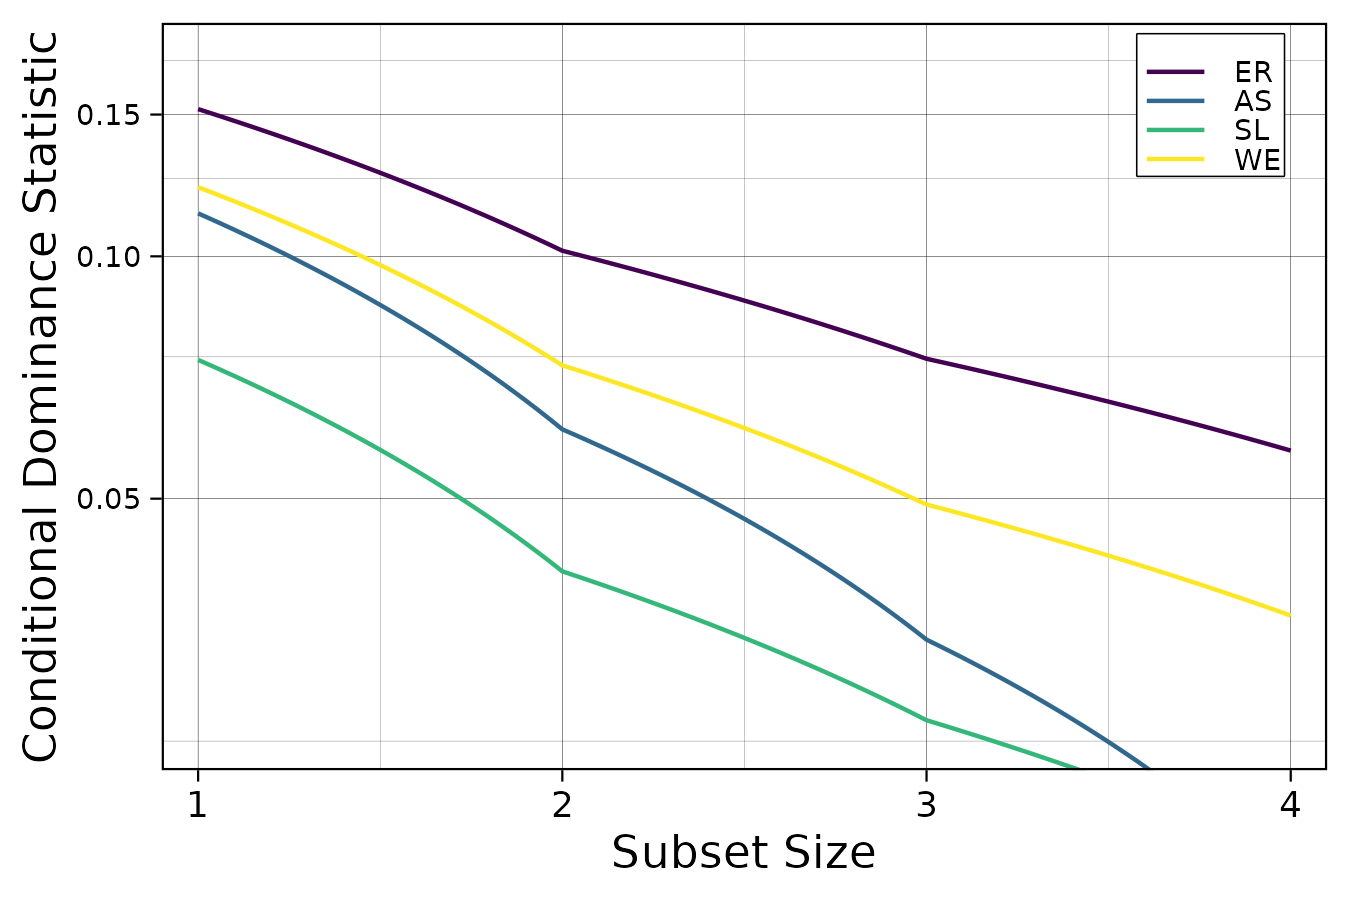
\includegraphics{includes/condit_gph}
	\end{longtable}

	Figure 1's results showed that a few conditional dominance designations were possible for both PR and NBR models.
	ER conditionally dominated AS, SL and WE. 
	In addition, WE conditionally dominated SL.
	By contrast, no conditional dominance relationships were possible with AS across both PR and NBR models as, for both models, AS starts with the second largest value at subset size of 1 and ends with the smallest value at subset size of 4.
	In part, this complex relationship has to do with AS's generally high correlations with other IVs. 
	At lower subset sizes, AS shows a larger value as its coefficient value is relatively large and its overlap with other IVs has not been taken into account.
	At higher subset sizes, AS's larger correlation with other IVs makes the increment it adds to prediction smaller as it overlaps with other IVs to a large extent.
	Thus, in combination, AS's pattern of intercorrelations produces a complex conditional dominance statistic trend.
	
	The example computation using ER above is extended here to compute conditional dominance statistics.
	The four conditional dominance statistics for ER are computed as:
	
	$$CDS^1_{ER} = R^2_{DEV_{ER}}$$
	
	$$CDS^2_{ER} = \frac{R^2_{DEV_{ER + AS}} - R^2_{DEV_{AS}}}{3} + \frac{R^2_{DEV_{ER + SL}} - R^2_{DEV_{SL}}}{3} + $$
	$$\frac{R^2_{DEV_{ER + WE}} - R^2_{DEV_{WE}}}{3}$$
	
	$$CDS^3_{ER} = \frac{R^2_{DEV_{ER + AS + SL}} - R^2_{DEV_{AS + SL}}}{3} + \frac{R^2_{DEV_{ER + AS + WE}} - R^2_{DEV_{AS + WE}}}{3} + $$
	$$\frac{R^2_{DEV_{ER + SL + WE}} - R^2_{DEV_{SL + WE}}}{3}$$
	
	$$CDS^4_{ER} = R^2_{DEV_{ER + AS + SL + WE}} - R^2_{DEV_{AS + SL + WE}}$$
	
	Each of the conditional dominance statistics are, again, components of the general dominance statistic computed above.
	
	Conditional dominance is a pre-requisite for the final designation between two IVs, complete dominance.
	Hence, it is only necessary to attempt to determine complete dominance for IVs where there is a conditional dominance designation.
	Recall that there were 4 conditional dominance designations above: WE conditionally dominated SL and ER conditionally dominated all other IVs. 
	The results in Table 4 show that all four IV comparisons produce complete dominance designations for the PR and NBR models.
	
	Complete dominance is determined by comparing $R^2_{DEV}$ from individual, comparable models.
	For the ER to AS determination this involved $R^2_{DEV_{AS}}$ compared to $R^2_{DEV_{ER}}$, $R^2_{DEV_{AS + SL}}$ compared to $R^2_{DEV_{ER + SL}}$, $R^2_{DEV_{AS + WE}}$ compared to $R^2_{DEV_{ER + WE}}$, and $R^2_{DEV_{AS + SL + WE}}$ compared to $R^2_{DEV_{ER + SL + WE}}$.
	For each of these four comparisons, the model containing ER was greater than the model containing AS.
	
	In conclusion, the DA results provide a set of dominance designations between the IVs indicating different levels of importance between them. 
	AS was, overall, the most important variable in terms of explaing the DV as reflected in the $E^2_{DEV}$ across PR and NBR models. 
	ER completely dominated AS, SL and WE.
	WE completely dominated SL, and generally dominated AS.
	Finally, AS generally dominated SL.

	\subsubsection{Section Summary}
	
	This section was intended to provide an extensive analytic of how to apply the recommended DA methodology using the $R^2_{DEV}$ to PR and NBR models.
	For these examples, estimated and interpreted model coefficients, their DA statistics, as well as provided schematics related to the computation of DA statistics.
	
	The data used in the modeling was simulated but was generated to be realistic and interpreted as though it was obtained empirically.
	As such, the data analytic examples above provided a valuable overview of recommended practice for computing DA statistics and determining DA designations with count DVs.
	
	The DA methodology discussed in the sections above grows more complicated when the count data meet specific conditions. 
	One condition discussed in the introduction is the condition where the observations in the data are "exposed" to the count generating mechanism differently.
	The section below shifts to discussing the conceptual underpinnings of these different exposure times for modeling and proceeds to discuss how such exposure times affect DA statistics and designations using an extension of the simulated data.
	
\section{Additional Consideration for CRMs}

	CRMs necessarily differ from other linear models as they have an implied level of aggregation that is associated with them.
	In fact, one interpretation of a Poisson distribution is as accumulated repeated sampling from a Binomial distribution with a set number of trials \cite(e.g.,){hodges1960poisson}.
	In this interpretation of the Poisson, the Poisson mean parameter $\mu$ is the product of the number of trials $n$ for the Binomial distribution times the probability $p$ of the event occurring in the Binomial distribution.
	Given the Binomial interpretation of the Poisson, it is clear that CRMs assume that the counts of events realized in the data are derived from Binomial processes that share the same number of trials and probabilities of occurrence.
	That is, CRMs assume that the realized counts stem from the same underlying Binomial processes.
	
	
	
	CRMs are able to accommodate adjustments where different Binomial processes are observed. 
	Below is a conceptual discussion of what these adjustments are, why they are important to apply, and how they affect DA statistics.

	\subsection{Exposure Variables and Offset Terms}
	
	The concept of exposure to a count generating process, as well as its importance to generating observed values, is easier to explain in the context of an example.
	Consider the following research question using a count DV.
	Does additional customer service training increase the number of positive reviews for a business?
	When thinking about research questions that are answered using CRMs, the Binomial interpretation of the Poisson is a convenient way to describe the parameter estimate results and how they are interpreted.
	A key interpretive question for this research is whether we believe that the training will affect the probability of receiving a positive review, the number of customers who can provide a review, or both factors.
	For this research question, the customer service training is likely to focus on the probability of receiving a positive review.
	Conceptually, the customer service training should, with a fixed set of customers, increase the count as the probability that any one customer is happy and thus provides a positive review is increased.
	These questions, focused on probability of the event occurring, are common in application to CRMs and are the focus of this discussion.
	
	Probability-oriented count DV questions are complicated by the nature of the data generation process as the same probability can produce different numbers of observed events with different numbers of trials or different levels of "exposure" to the probability.
	For example, two business locations might have 10 positive reviews each but one may have had 1,000 customers and the other 100 customers.
	Both observations yield the same count value but imply starkly different probabilities of observing an event (i.e., $\frac{10}{1000} = .01$ and $\frac{10}{100} = .1$).
	In this case, the number of customers is a nuisance factor that obscures the underlying probability of occurrence of the sought after event.
	
	CRMs can control for such nuisance/unequal exposure to the count generating mechanism using what is known as an \emph{offset} term.  
	The offset term is usually assumed to be a natural log transformed version of the exposure variable and enters into the CRM with a coefficient of 1.
	The coefficient of 1 results in the count DV being transformed into a rate dependent on values of the exposure variable.
	How the count DV is transformed into a rate with a coefficient of 1 follows from the following algebraic manipulations.
	Imagine a simple case where an intercept only model is fit with an offset.
	In a log-linear CRM, this produces: $y = e^{offset + \beta}$.
	Recall that the offset term is the natural log of a variable, say, $o$.  
	Applying the natural log and substituting $\ln o$ for $offset$, the prior equation can be written as $\ln y = \ln o + \beta$.
	Re-arranging the $\ln o$ term results in $\ln y - \ln o = \beta$ which, given the properties of logarithms, is tantamount to $\ln \frac{y}{o} = \beta$.
	Therefore, the inclusion of a natural log transformed exposure variable turns the count DV into a rate that depends on exposure variable forced into the model as an offset term.
	
	The re-scaling of the DV by the offset term adjusts for differences in Binomial trials between observations in a count DV and better reflects the underlying probability which is desirable for probability-based research questions with CRMs.
	The re-scaling process also reduces the extent of unexplainable variation, or deviance, in the count DV as observations with high counts and high exposure values are pulled nearer those with low counts and low exposure values.	
	As a result, inclusion of an offset term will affect $R^2_{DEV}$ values and DA statistics on which they are based.
	It is also important to note that the relationships IVs have with the exposure variable can have a substantial impact on the estimated coefficients an DA statistics that can bias results and affect inference for probabilty-oriented count research questions.
	
	The sections below extend the modeling discussed above by describing the generation of two new variables that have different patterns of exposure to the count generating process. 
	The modeling process above is then repeated on these new variables to illustrate the effect that exposure variables, and modeling them as offset terms, have on both modeling and DA results.
	
	\subsection{Dominance Analysis with Offset Terms: Analytic Examples}
	
	This section is an extension of the data analysis section above that discussed the PR and NBR modeling.
	Here, an additional two Poisson distributed variables are created that have different levels of exposure to the count generating process and different relationships with the IVs.
	
	The next section provides a description of the variables and how they were generated. Full details on data generation are available in the online supplement.
	
		\subsubsection{Data Generation}
		
	The data described in this section extended on the generated data produced for the analytic examples discussed previously.
	These data were then generated with the intention to balance their "realism" with built-in properties that illustrate the nature of the exposure effects.
	
	The data simulated in this section again focused on the 6,780 tailors generating stock jackets in a fortnight.
	One key difference from the data above is that the period of time in which these data simulated was for two different local holidays.
	The first stock jacket variable occurred for near a religious holiday (SJ\_RH) that is not celebrated in the same way by all tailors.
	The observation of this religious holiday produced inconsistent leaves of absence, and thus less exposure, across tailors that were uncorrelated with their IV values.
	
	The second stock jacket variable occurred near a common time when tailors take voluntary holidays (SJ\_VH) that depends on tailor workload.
	Because tailors who produce more jackets are more likely to have their workload sufficiently light to take the holiday, the IVs are inversely related to the likelihood of taking holiday time and thus exposure.
	The sport jacket variable was otherwise identical to the previous version discussed above. 
	The exposure days for religous holidays (RH) and voluntary holidays (VH) ranged from a minimum of 1 working day to 10 (i.e., all working days in a fortnight) and were uniformly distributed.
	
	The means, standard deviations, and correlations with the IVs and one another are reported in Table 6.
	
	\begin{longtable}{lrrrrrr}
		\caption*{
			{\large Table 6: Descriptive Statistics}
		} \\ 
		\toprule
		&  &  Standard & \multicolumn{4}{c}{Correlations} \\ 
		\cmidrule(lr){4-7}
		Variable & Mean & Deviation & ER & AS & SL & WE \\ 
		\midrule
		SJ\_RH & $0.5447$ & $0.7575$ & $0.3455$ & $0.3247$ & $0.2773$ & $0.3174$ \\ 
		RH & $5.5186$ & $2.8950$ & $-0.0108$ & $-0.0072$ & $-0.0156$ & $-0.0249$ \\ 
		SJ\_VH & $0.4709$ & $0.6549$ & $0.2332$ & $0.2325$ & $0.1631$ & $0.2405$ \\ 
		VH & $5.5301$ & $2.8897$ & $-0.3952$ & $-0.3450$ & $-0.3574$ & $-0.3252$ \\ 
		\bottomrule
	\end{longtable}
	
	Table 6 shows that the means and standard deviations for SJ\_RH and SJ\_VH were effectively identical but had shrunk from the value of SJ in Table 1.
	This is because SJ implicitly assumes an exposure value of 10 for all observations. 
	Because the exposures for SJ\_RH and SJ\_VH were both around 5.5 days, their means shrunk proportional to the number of days of exposure.
	If 10 days produces a mean of 1, then 5.5 average days should produce an average of .55.
	
	The pattern of correlations between the SJ-exposed variables and their exposures with the IVs is also of note. 
	In the case of both SJ\_RH and SJ\_VH, their correlations with the IVs are smaller than SJ as reported in Table 1. 
	This is due to a restriction in variance from reduced exposure time to the count generating process for these variables.
	Note also the differences between RH, the exposure variable for SJ\_RH, and VH, the exposure variable for SJ\_VH.
	RH is, as expected, effectively uncorrelated with the IVs.
	By contrast, VH shows strong, negative correlations with the IVs.
	It is these negative correlations that produce an additional suppressing effect on the correlations between SH\_VH and the IVs as the restriction in variance due to exposure is inversely related to counts.
	These negative correlations are also the reason SJ\_VH's mean is less than  the expected value of .55.
	
	In sections to come, the new SJ\_RH and SJ\_VH variables are analyzed in separate PR models.
	Both models are evaluated with and with out the use of their exposure variable modeled as an offset.
	The results below are subdivided by the type of exposure variable and begins with SJ\_RH, the uncorrelated exposure variable.
	
		\subsubsection{Uncorrelated Exposure Variable}
		
	The two models using SJ\_RH, one with and one without the exposure variable modeled with an offset, are reported in Table 7.
	Only coefficient and IRR values are reported in Table 7 as their values are the focus of this discussion.
		
	\begin{longtable}{l|rrrr}
		\caption*{
			{\large Table 7: Uncorrelated Exposure Poisson Regression}
		} \\ 
		\toprule
		\multicolumn{1}{l}{} & \multicolumn{2}{c}{No Offset} & \multicolumn{2}{c}{Offset} \\ 
		\cmidrule(lr){2-3} \cmidrule(lr){4-5}
		\multicolumn{1}{l}{} & Coefficient & IRR & Coefficient & IRR \\ 
		\midrule
		Inter & $-0.8170$ & $0.4418$ & $-2.5276$ & $0.0799$ \\ 
		ER & $0.2575$ & $1.2937$ & $0.2657$ & $1.3043$ \\ 
		AS & $0.1521$ & $1.1643$ & $0.1502$ & $1.1621$ \\ 
		SL & $0.1455$ & $1.1566$ & $0.1515$ & $1.1636$ \\ 
		WE & $0.1271$ & $1.1355$ & $0.1347$ & $1.1442$ \\ 
		\bottomrule
	\end{longtable}
	
	Table 7 shows that the coefficients and IRR values for the models with and without an offset term are very similar to one another with the exception of their intercept value.
	That the exposure variable does not noticeably affect the magnitude of the coefficients, despite the clear impact the exposure variable has on the SJ distribution's mean and variance relative to when there is no exposure effect, may come as a surprise.
	Indeed, the exposure variable works in a similar way to random/uncorrelated error variance which tends to shrink the magnitude of coefficients in LRM.
	The key difference between error variance in LRM and 'random' exposure variables in CRMs is the multiplicative nature of the CRM's coefficients.
	For an LRM, the additional error variance dilutes what a 1 unit change in an IV does in terms of units of change to the DV.
	For a CRM, the interpretation of the coefficient is that a 1 unit change in an IV does in terms of a percent change to the DV.
	Here the random variation from an exposure variable would have affect change disproportionately across levels of the DV to shrink the magnitude of the coefficients in the same way as in an LRM.
	
	Compared to the coefficients, the intercept across both models does show substantial change with the addition of the offset term.
	The difference across the offset and no offset models is to re-scale the mean value in a way that reflects the new interpretation of the DV when an offset is estimated.
	The effect of the re-scaling is clearest when comparing IRR values across models.
	The IRR value for the no offset model is .4418, which is an IV-adjusted mean based on the .5447 mean value for SJ\_RH.
	The IRR value for the offsets model is .0799, which is an IV-adjusted rate based on the theoretical underlying rate of .1000.
	This theoretical rate is obtained from for SJ which is what SJ\_RH would be equivalent to given no exposure differences.
	In this case, SJ's mean is 1 and implied exposure is 10 working days.
	The rate of counts for SJ is then $\frac{1}{10}$ or .1000.
	Thus, the offset term has, as expected, re-scaled the DV from a count to a rate.
	
	It is also important to note that the coefficient values obtained for the IVs for both models in Table 7 are, again with the exception of the intercept, similar to the values obtained for the non-exposure affected SJ variable in Table 2.
	Whereas the effects of differential exposure that are uncorrelated with the IVs has had a minimal effect on the estimated coefficients, the effect of uncorrelated differential exposure is more noticeable among the next set of results; the general dominance statistics for both models reported in Table 8.
	
	\begin{longtable}{l|rr}
		\caption*{
			{\large Table 8: Uncorrelated Exposure Poisson-based General Dominance Statistics}
		} \\ 
		\toprule
		\multicolumn{1}{l}{} & No Offset & Offset \\ 
		\midrule
		ER & $0.0708$ & $0.0863$ \\ 
		AS & $0.0541$ & $0.0641$ \\ 
		SL & $0.0437$ & $0.0545$ \\ 
		WE & $0.0551$ & $0.0698$ \\ 
		\midrule
		Overall & $0.2238$ & $0.2748$ \\ 
		\bottomrule
	\end{longtable}
	
	Table 8 shows that the general dominance statistics for models with the offset term are all larger than their corresponding values without the offset term. 
	However ostensibly different, the differences in magnitudes between these results is due to the differences across models in the magnitude of the $R^2_{DEV}$ from which each IV has been partitioned.
	In fact, the relative proportions of the $R^2_{DEV}$ explained by each of IVs within each model is nearly identical.
	For example, ER is responsible for approximately 31\% of the $R^2_{DEV}$ for both models (i.e., $\frac{.0708}{.2238} = .3164; \frac{.0863}{.2748} = .3140)$.
	The reason for the notable difference in explained deviance across models is because of the offset term's role in reducing unexplained variation in the DV for probability-based research questions.
	As was discussed previously, the exposure effect produces variation in the count DV that is unrelated to the focal probability of the occurrence of an event.
	The inclusion of the offset term reduces this unexplained variation directly and obtains results that are closer to those that would be obtained if exposure was equal.
	To this last point, note that the general dominance statistics and $R^2_{DEV}$ for the offset model are much closer to the results of SJ in Table 5 than are the no offset model's results.
	
	The section below moves to discussing the results of the use of exposure terms for the SJ\_VH variable in which the IVs are related to exposure.
	As with the results for SJ\_RH, the models with and without offset terms are reported.
	
		\subsubsection{Correlated Exposure Variable}
		
	The no offset and offset models using SJ\_VH are reported in Table 9.
	As before, only the coefficient and IRR values from each model are reported.
	
	\begin{longtable}{l|rrrr}
		\caption*{
			{\large Table 9: Correlated Exposure Poisson Regression}
		} \\ 
		\toprule
		\multicolumn{1}{l}{} & \multicolumn{2}{c}{No Offset} & \multicolumn{2}{c}{Offset} \\ 
		\cmidrule(lr){2-3} \cmidrule(lr){4-5}
		\multicolumn{1}{l}{} & Coefficient & IRR & Coefficient & IRR \\ 
		\midrule
		Inter & $-0.8512$ & $0.4269$ & $-2.5182$ & $0.0806$ \\ 
		ER & $0.1638$ & $1.1780$ & $0.3054$ & $1.3572$ \\ 
		AS & $0.1145$ & $1.1214$ & $0.1735$ & $1.1895$ \\ 
		SL & $0.0642$ & $1.0663$ & $0.1668$ & $1.1815$ \\ 
		WE & $0.1118$ & $1.1182$ & $0.1568$ & $1.1698$ \\ 
		\bottomrule
	\end{longtable}
	
	As compared to the uncorrelated exposure results in Table 7, the correlated exposure results show different patterns of results across no offset and offset models for all IVs.
	Whereas the offset model looks relatively similar to the pattern of results from the no offset model in Table 7 as well as the results in Table 2, the no offset model shows a notable shrinkage in the magnitude of the coefficient and IRR for SL and AS relative to other results.
	The magnitude of SL's coefficient across all models has been between AS and WE whereas for no offset model using SJ\_VH, SL's value is notably lower than all other coefficients.
	AS' coefficient in the no offset model is also relatively smaller than in all other models to this point; nearly equal in value to WE's coefficient value.
	... note sim of intercept...
	
	The no offset model results in Table 9 show the biasing effect of the correlated exposure variable on coefficient estimates when it is not modeled as an offset.
	The notable change to coefficients due to the correlated exposure are likely to impact DA results as well.	
	Table 10 below reports on the general dominance statistics derived from both models in Table 9.
	
	\begin{longtable}{l|rr}
		\caption*{
			{\large Table 10: Correlated Exposure Poisson-based General Dominance Statistics}
		} \\ 
		\toprule
		\multicolumn{1}{l}{} & No Offset & Offset \\ 
		\midrule
		ER & $0.0307$ & $0.0889$ \\ 
		AS & $0.0280$ & $0.0656$ \\ 
		SL & $0.0127$ & $0.0512$ \\ 
		WE & $0.0342$ & $0.0737$ \\ 
		\midrule
		Overall & $0.1055$ & $0.2795$ \\ 
		\bottomrule
	\end{longtable}

	Table 10's results show, similar to those of Table 9, that the model including an offset is very similar to the results obtained from the offset model in Table 7 as well as SJ's results from Table 5.
	Thus, the effect of a correlated exposure variable is relatively minimal on DA statistics given that the appropriate offset term is included in the model and reproduces results similar to a model not affected by differential exposure.
	By contrast, the no offset model shows both a large reduction in the magnitude of the $R^2_{DEV}$ as well as a change in the rank orders of the IVs.
	The reduction in the magnitude of the $R^2_{DEV}$ was produced, in part, for reasons similar to the uncorrelated exposure models as additional unexplainable variation was added to the count DV. 
	In the case of the correlated exposure model, the extra variation in counts due to differential exposure also affected coefficient estimates as can be seen in Table 9.
	In all cases, the estimated magnitude of the IV's coefficients, when affected by differential exposure that was correlated with the IVs, was smaller than expected relative to the models without such differential exposure.
	The effect of correlated, differential exposure also changed the rank order of top two IVs.
	In the no offset model, WE obtains the highest general dominance statistic value followed by ER.
	The correlations in Table 6 reveal the probable reason for this effect in that WE both has the highest relationship with SJ\_VH as well as the lowest correlation with the exposure variable VH.
	Hence, without the offset term adjustment, WE appears to have the strongest overall impact on SJ\_VH.
	
		\subsubsection{Section Summary}
		
	This section has discussed the effects of unequal exposure to a count generating process on both estimated coefficients as well as DA statistics.
	When unequal exposure to the count generating process is uncorrelated with the IVs in the model, the effect of unequal exposure is minimal, mostly changing the total $R^2_{DEV}$ value obtained as well as the model intercept.
	When unequal exposure to the count generating process is, at least in part, determined by the IVs in the model, the effect of unequal exposure is far more influential.
	The results in Tables 9 and 10 show that correlated, unequal exposure can bias coefficient estimates as well as explained deviance metrics, as well as change the rank order of IV importance.
	
	Although unequal exposure can have notable biasing effects, such biases can be corrected for using the exposure variable as an offset term in the model.
	Modeled offset terms do not necessarily recover the effect of each IV that would have been obtained had there been no unequal exposure, but do result in notable improvements to the model estimates and DA statistics over the alternative where an offset term is not modeled. 
	These results then show the importance of considering whether it is possible that observed counts in a CRM could result from different probabilities of the event occurring, different exposure to the count generating probability, or both.
	If it is the case that both factors might be producing counts and the focus of the research question is on the probability of events, it is important to attempt to model the exposure variable as an offset term to avoid potential bias in the results.

	
\section{Discussion}

	This manuscript provided a rationale for application of a specific methodology when using relative importance analysis with CRMs.
	I argue that DA, as an extension of Shapley value decomposition, is an applicable method to CRMs and in addition provided a fit metric for use in the relative importance analysis of any CRM.
	Specifically, I recommend the use of the deviance $R^2$ or $R^2_{DEV}$ as it is directly analogous to the explained variance $R^2$ or $R^2_{EXP}$.
	Applying the $R^2_{DEV}$ to CRMs then follows directly from the application of $R^2_{EXP}$ to LRM.
	
	In addition, this manuscript provides a discussion of one specific data analytic consideration of particular relevance to CRMs; differential exposure to a count generating process.
	In the discussion of this issue, I outline its relevance to the evaluation of count DV-based research questions and showed examples of how the concept affects both model coefficient estimates as well as DA statistics.
	The section focusing on differential exposure also showed the extent to which modeling such differential exposure variables as offset terms could correct the biasing effect and produces more accurate estimates of parameters and DA statistics.
	
	In combination, the discussion of these issues supplies organizational scientists with the tools necessary to accurately evaluate IV relative importance as applied to a series of widely used CRMs. 
	It is important when modeling count DVs that the recommendations provided by Blevins et al. \citeyear{blevins2015count} are considered first as their guidance can point a researcher to the appropriate model to apply to the data. 
	This article seeks only to pick up where they left off and recommend practices for the evaluation of the selected CRM after estimation. 
	
	This article touched on many of the key aspects necessary for extending DA to CRM.
	Below I discuss additional potential extensions of this work and future directions for the evaluation of IV importance in organizational science.
	
	\subsection{Extensions and Future Directions}
	
	PR in particular, but also NBR, are instances of the broader class of models known as generalized linear models \cite{mccullagh2019generalized}. 
	Specifically, PR is a generalized linear model in the Poisson "family" with a natural lograrithm "link" \cite(See implementation of generalized linear models in R;){R}.
	In extending DA to CRMs, I also effectively make an argument for the applicability of DA using the $R^2_{DEV}$ to \emph{any} generalized linear model using the same approach.
	That is, given that DA is applicable to CRMs, it is also applicable to any generalized linear model with a different distribution family or link function.
	This is an important point to note as it is not necessary for researchers to hesitate in applying DA to generalized linear models that have not been explicitly discussed in the literature.
	Indeed, because this article links Shapley value decompsition to DA and then provides a method for implementing DA with a specific generalized linear model (i.e., CRMs), it is trivial to extend the same approach to a generalized linear model with a different family and link function.
	Therefore, DA with the $R^2_{DEV}$ approach is applicable to any generalized linear model.
	
	It is worth noting before moving on that the $R^2_{McFadden}$, recommended by Azen and Traxel \citeyear{azen2009using} for use in DA with logistic regression generalized linear model, is equivalent in computation to the $R^2_{DEV}$. 
	This is because the form of the deviance computation for a logistic regression produces a value that is  a scalar multiple of its log-likelihood. 
	As such, the perspective taken in the paper agrees with that of the past research in that recommends the use of $R^2_{McFadden}$. 
	Additionally, Cameron and Windmeijer \citeyear{cameron1996r} note that the $R^2_{McFadden}$ differs from the $R^2_{DEV}$ by a scalar multiple and is valid in application to CRMs and, by implication, the computation of DA statistics using CRMs.
	
	Shapley value decomposition and, by extension, DA are well-known to be computationally expensive methodologies that require averaging of contributions by IVs to a model over a potentially extremely large pool of values.
	For example, a DA with 20 IVs would require $2^{20} = 1,048,576$ different sub-models in order to collect fit statistics associated with all possible combinations of IVs and compute general dominance statistics.
	Whereas modern computing power could feasibly accommodate around one million models in a reasonable amount of time, adding additional IVs beyond 20 continues to grow the number of required models geometrically. 
	An additional 10 IVs results in $2^{30} = 1,073,741,824$ or over one billion model required to obtain dominance statistics; even if each CRM took $\frac{1}{100}$ of a second to estimate, this many models would take nearly 4 months to complete on a single machine.
	
	Many approaches have been developed to approximate Shapley values/DA that are far less computationally expensive. 
	Relative weights analysis \cite{johnson2000heuristic} is a commonly applied alternative to DA that approximates the averaging process between all possible models using singular value decomposition.
	Relative weights analysis has shown some promise in past research \cite{lebreton2007multidimensional}, and has been extended to one generalized linear model in published research \cite[i.e., logit regression]{tonidandel2011relative} but has been subject to sharp criticism \cite{thomas2014johnson} and is not among commonly recommended methods for relative importance of linear models \cite{gromping2007estimators}. 
		
	Shapley values have also grown in use among methodologists seeking an approach that can provide "interpretable machine learning" results \cite{molnar2020interpretable}.
	In many cases, such efforts apply Shapley values, or approximations to them, that decompose predicted values for each observation in the data \shortcite(e.g.,){lundberg2020local}.
	Such Shapley decompositions of predicted values can be used, when cross-referenced with a observations' IV values, that, in the aggregate, can be used to get a sense for the nature of the effect of that IV on the DV much like a coefficient in a CRM.
	Machine learning models often have a great number of IVs which makes the "exact" computation of Shapley values infeasible.
	Methods to facilitate Shapley value computations in the literature have included sampling permutations \cite{castro2009polynomial} and normal approximations under specific assumptions \cite{fatima2008linear}, among others.
	In application to machine learning methods, Shapley value approximations have often use a weighted-least squares approximation with sampling and adjustments for dependence \cite{sellereite2020shapr,aas2021explaining}. 
	Such approximation methods may be useful in application to CRM and other models as an alternative estimator of the DA statistics.
	
	Finally, to the knowledge of the author, there has been relatively little work has considered the value in applying Owen decomposition \cite(e.g.,){huettner2012axiomatic} to DA broadly.
	Owen decomposition differs from Shapley in that a grouping structure is applied to IVs in which groups of IVs "negotiate" values jointly between groups but subsequently also "negotiate" values within their group as well. 
	The result is that each IV obtains a component of the fit metric, and the Owen values are a full decomposition of the fit metric, but a large number of sub-models can be eliminated. 
	For example, by grouping 8 IVs into 4 groups of 2, the number of sub-models needing estimation goes from $2^8 = 256$ to $2^4 + 2^2*4 = 32$---an eight-fold reduction in the number of sub-models needing estimation.
	An approach such as this can directly (i.e., without approximation) and substantially reduce the size of the pool of sub-models to estimate and retains feasibility for computing dominance designations such as complete dominance.	
	
	\subsection{Limitations}
	
	This work provides a justification for why DA is applicable to CRMs and offers multiple, extensive data analytic examples that model and dominance analyze simulated data.
	The data simulated in this manuscript were designed to have specific properties that make them applicable to the different CRMs and CRM-specific data analytic issues that were valuable to discuss as applied to DA.
	The use of simulated data is not, in and of itself, a limitation.
	The limitation in using simulated data is in avoiding many of the decision points noted by Blevins et al. \citeyear{blevins2015count} related to the selection of the appropriate CRM.
	Careful consideration of the decision to choose a specific CRM is important, but were avoided in this work to focus on modeling and DA with data that were unequivocally known to apply to specific models.
	In addition to not covering the model selection process, I also acknowledge that using simulated data adds additional complexity to following along with the methodology in the online supplement.
	The procedures used to simulate the various count DVs are complex but could add value to understanding count DVs for interested readers with a working knowledge of R \cite{R}.
	
	In addition, this manuscript provides two examples of how omitting a relevant offset term can result in unexpected changes to DA statistics and designations.
	The examples provided show how the omission of an offset term affects DA statistics in ways different from, and arguably more serious than, estimated model coefficients.
	The purpose of this section was to raise awareness of this issue as one that has received less attention among organizational scientists but has the potential to strongly affect importance designations.
	This manuscript makes no attempt to quantify or characterize the extent of bias that can occur when omitting an offset term as I consider doing so out of scope.
	Although a thorough evaluation of the potential bias introduced by omitting an offset term was not undertaken in this work, I see future research focusing on this issue as applied to DA of potential value and help researchers identify situations when such bias is more or less likely to occur.
	An evaluation of omitted offset terms could be taken on in a way similar to Braun, Converse, and Oswald's \citeyear{braun2019accuracy} evaluation of measurement reliability and sampling error on dominance statistics in meta-analytic LRM.
	
	Related to sampling error, prior work on DA has also suggested the application of bootstrapping to estimate standard errors for general dominance statistics and reproduce-ability values for dominance designations \cite{azen2009using,braun2019accuracy}. 
	Bootstrapping the dominance statistics and designations is possible for CRM-based DA in the same way as was outlined for logistic regression by Azen and Traxel \citeyear{azen2009using} but is not examined in the present work.
	A severe complication with the bootstrapping method as applied to DA is, as discussed above, that as the number of IVs increases, the DA itself becomes computationally infeasible---let alone the entirety of the DA process being repeated for a fixed number of bootstrap iterations.
	A useful extension on this research would be to evaluate approximations to a full DA-with-bootstrapping process that could provide information on sampling variability but would remain scale-able and computationally feasible with CRMs (and other predictive models) of typical sizes encountered in the literature.
	
	Finally, this work does not directly address how to conduct DA with a commonly observed complication with count DVs, zero inflation.
	Zero inflation is a condition where the count DV shows more zero counts than would be expected from a standard Poisson or negative Binomial distribution \cite(e.g.,){blevins2015count}. 
	A zero-inflated model is often thought of as having an "opt out" process that forces counts to 0 owing to making them not possible. 
	For example, as applied to the generation of stock jackets, if a process in which tailors shops had to close and thus could not produced any jackets was modeled, such IVs could be modeled in a zero-inflation model to recover the effects of the other predictors on the "count" process.
	An additional complexity that results from zero-inflated models is that it is possible to allow IVs to predict the count generating process, the opting out process, or both.
	In such circumstances the researcher may have to consider whether an alternative approach that emphasizes parameter estimates as opposed to IVs is better suited to the importance determination with DA; indeed, past work has used zero-inflated Poisson regression as an example of the application of parameter estimate-based DA \cite{luchman2020relative}.
	I expect that the recommendations offered in this paper could extend in a straightforward way to zero-inflated models as Cameron and Windmeijer \citeyear{cameron1996r} do consider zero-inflated models in terms of $R^2_{DEV}$ computation. 
	Such extensions would still need to consider whether IV- or parameter estimate-based DA fits the research question they are asking of the zero-inflated model.
	
	
	\subsection{Conclusion}
	
	DA is a useful post-estimation methodology for determining the importance of IVs in statistical models such as CRMs.
	This manuscript has provided argumentation for how and why DA could extend to CRMs, offered extensive examples focusing on the computation of DA statistics with simulated data, and provided recommendations for how to adjust a CRM-based DA when observations in the count DV may have different levels of exposure to the count generating process.
	
	In combination, the content of this manuscript will provide organizational and other behavioral scientists the necessary steps for determining the relative importance of IVs in CRMs they estimate.
	It is also important to note that several software implementations that can accommodate CRMs are available in different software.
	For instance, the \texttt{domin} package in Stata \cite{luchman2021determining} as well as the \texttt{parameters} \cite{ludecke2020extracting} and \texttt{domir} packages in R \cite{luchman2022package} can accommodate CRMs. 
	Thus, combined with this article's recommendations, all the necessary tools for the DA of CRMs are available to researchers to better understand their count DV-based models.


\bibliography{CountDominance.bib}
\bibliographystyle{mslapa}
	
\end{document}